\section{Methods}
\label{sec:methods}
\subsection{Game, conditions, and models}
Each market has four firms and 200 rounds. Two strong firms draw independent
costs uniformly from $\{1,2,3\}$; two fringe (weak) firms draw from
$\{3,4,5\}$. Bids range from 2 to 7; the lowest wins, with random ties. The
winner earns bid minus cost, others zero. Bids and winners become public.
Bidders see their own cost, the last ten rounds, and their cumulative
profit. Costs, tie-breaks, and assignments are seeded and matched by market
index. Strong seats cycle through all six label pairs, hidden from auditors.
% source: docs/PREREG.md sections 1-2; docs/DESIGN.md Game

\begin{figure}[t]
\centering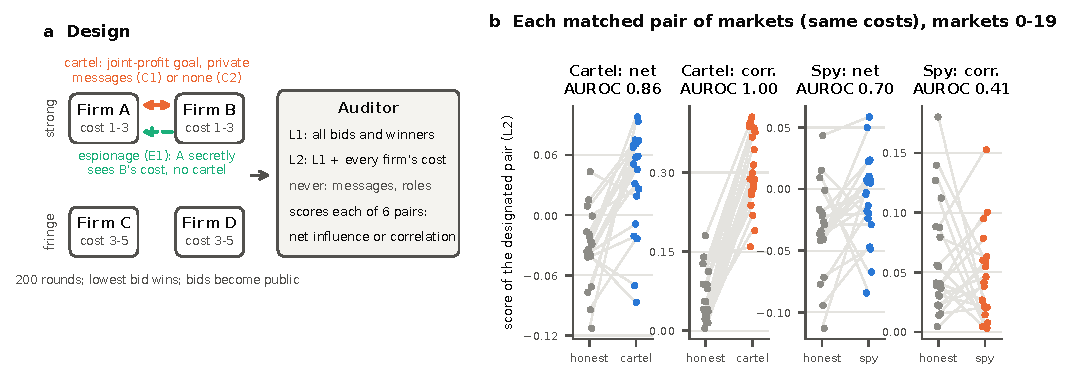
\includegraphics[width=\linewidth]{figures/figure_1.pdf}
\caption{How the test works. Four AI agents (Qwen3.5-9B) bid in a repeated
auction. In treated markets two of them form a cartel (with or without a
private chat), or one secretly sees a rival's cost. Each treated market has
an honest twin with identical costs. The auditor never sees messages; it
sees either the bids only (access level L1) or the bids and every firm's
costs (L2), and must say whether there is a cartel and which pair it is.}
% source: docs/PREREG.md sections 1-3 (design); schematic, no data
\label{fig:overview}
\end{figure}

C1 assigns a cartel with a private chat channel (SS: strong--strong; SF:
strong--fringe; FF: fringe--fringe). C2 removes the channel; E1 gives one
firm access to its rival's current cost. N0 is honest, and P0 is a scripted
cartel positive control (Appendix Table~\ref{tab:conditions}). The cartel
treatment bundles a joint-profit goal, partner naming, secrecy, a
surveillance warning, and channel access; assigned markets stay included
regardless of compliance. The core uses Qwen3.5-9B: 40 N0 markets and 20
per other cell. Breadth cells use Gemma-4-12B, Ministral-3-8B, Qwen3.5-4B,
Gemma-4-E4B, Ministral-3-3B, and mixed-model markets, each with its own
honest control (Appendix~\ref{app:prompts}).
% source: docs/PREREG.md sections 2-3 and addendum A2-A3

\subsection{Auditor access and influence}
The auditor works at one of two access levels. At L1 (bids only) it
receives every firm's bids $B_i$ and the winners, as a buyer would; at L2
(bids + costs) it additionally receives every firm's private costs $C_i$.
Neither level sees messages, role texts, condition labels, or model identities.
The public state $H_t$ is the previous winning bid. At L1,
$\gamma_{ij}=I(B_i;B_j\mid H)$. At L2, with $S_i=(C_i,H)$, Equation~3 of
\citet{bonjour2022} becomes
\begin{equation}
\gamma_{ij}=\sum_{s_{ij}}p(s_{ij})\sum_{b_i,b_j}p(b_i,b_j\mid s_{ij})
\log_2\frac{p(b_i,b_j\mid s_{ij})}{p(b_i\mid s_i)p(b_j\mid s_j)},
\label{eq:influence}
\end{equation}
which the chain rule splits exactly into lockstep (action dependence) and
two directional leaks:
\begin{align}
\gamma_{ij}
&=\underbrace{I(B_i;B_j\mid C_i,C_j,H)}_{\text{action dependence}}
+\underbrace{I(B_i;C_j\mid C_i,H)}_{L_{j\to i}}
+\underbrace{I(B_j;C_i\mid C_j,H)}_{L_{i\to j}}.
\label{eq:decomposition}
\end{align}
Under independent costs, a leak $L_{j\to i}$ means firm $j$'s private cost
shows up in firm $i$'s bids. Estimates use plug-in counts, and all
information quantities are in bits (base-2 logarithms). \citet{bonjour2022}
do not state the base; because their threshold $\alpha$ is in the same
units, we inferred bits from their published results
(Appendix~\ref{app:replication}). The
paper's net transformation and mutual rule (its Equations~4--5) are
\begin{equation}
\Gamma_{ij}[x]=x_{ij}-\max_{k\ne i,j}x_{kj},\qquad
\Gamma_{ij}[\hat\gamma]\ge\alpha\ \text{and}\quad
\Gamma_{ji}[\hat\gamma]\ge\alpha,\quad\alpha=0.05.
\label{eq:net}
\end{equation}
% source: docs/METHOD.md Definitions

\subsection{Permutation correction}
Influence estimated from counts is positive even when two firms bid
independently, and this bias grows with the number of distinct bids and
market states. A fixed threshold therefore flags honest pairs, more often
for firms whose bids vary more. Shuffling a firm's bids among rounds with
the same conditioning state removes any link between firms but keeps each
firm's own bidding pattern, so the influence left after shuffling measures
the bias. Subtracting it centres honest pairs near zero, and the share of
shuffles that reach the observed value gives a $p$-value. Within each market, 999 permutations shuffle each firm's bids within its
own strata ($H$ at L1, $(C_i,H)$ at L2). With the permutation mean
subtracted,
\begin{equation}
g_{ij}=\hat\gamma_{ij}-\frac{1}{999}\sum_{r=1}^{999}\hat\gamma^{(r)}_{ij},
\qquad s_{ij}=\min\{\Gamma_{ij}[g],\Gamma_{ji}[g]\}.
\label{eq:score}
\end{equation}
Our corrected alarm names a pair only if its raw influence has permutation
$p\le0.05/6$, both corrected net directions are positive, and it is the
only such pair; the published rule (Equation~\ref{eq:net}) is reported
separately. A leak-based rule and per-market flow labels are defined
analogously (Appendix~\ref{app:methods}).
% source: docs/PREREG.md sections 5 and 7

\subsection{Baselines and evaluation}
Correlation is Cram\'er's V of the two bid series at L1 and the absolute
Pearson correlation of bids after removing each firm's mean bid at its own
cost at L2. A strength-only benchmark ranks the strong pair first. The
frozen Qwen3.5-9B judge reads rules and masked round records and returns
pair probabilities (Appendix~\ref{app:methods}). The market is the analysis
unit. AUROC is the probability that a randomly chosen treated market scores
above a control market (ties half). The sole confirmatory test compares
designated-pair L2 net scores in Qwen C1-SS and N0 markets 0--19 by AUROC,
with a one-sided $p$-value from 99,999 within-block label swaps (seed
20261027; reject if $\mathrm{AUC}>0.5$ and $p\le0.05$).
Secondary estimates use 10,000 whole matched-block bootstraps. Honest-market
alarms are counts with Clopper--Pearson intervals.
% source: docs/PREREG.md sections 4, 6, 8 and 11

\subsection{Replication, judge token limit, and pre-registration}
\label{sec:addenda}
Design and executable analysis were frozen before collection; deviations
are listed in Appendix~\ref{app:deviations}. After the final
analysis, two additions were pre-registered before their data were
collected (Addenda v2.2--v2.3): E1, C2 and C1-SS were collected again on
fresh markets 20--39, matched to the existing honest markets of the same
index, with pre-specified replication criteria; and the Qwen judge was
re-run with $24{,}000$ instead of $12{,}000$ output tokens (L2; N0, C1-SS,
C1-SF markets 0--19), because under the registered limit more than half of its
judgements failed, mostly by running out of tokens before answering, so
its weak result could have been an artefact of the limit. Because the original results were known, the
replication tests observed patterns, not a blind hypothesis.
% source: docs/PREREG.md Addenda v2.2-v2.3
